%Chapter 5 - Current state of the MEGA65 project
%What is the current state of the MEGA65 project?

\chapter{Current state of the MEGA65 project as of March, 2019}
\label{cha: Chapter5}
This chapter discusses the current state of the MEGA65 project in both its form-factors: the MEGAphone hand-held console and the desktop form-factor. 
%----------------------------------------------------------------------------------------
%----------------------------------------------------------------------------------------
\section{FPGA-based architecture}
The core of both form-factors of the MEGA65 is the FPGA-based components, such as the CPU and video controller, designed by Dr. Paul Gardner-Stephens. The FPGA components are practically complete, with Detlef suggesting a 99\% compatibility with Commodore 64 software. Achieving the last 1\% may be as hard as achieving the previous 99\% though, as such it may not be worth the time to achieve full 100\% compatibility. There are still some bugs present in the FPGA components which need to be addressed.

The CPU is an 8-bit enhanced 6502 microprocessor called a GS4502. It currently doesn't support all of the illegal 6502 opcodes, meaning it cannot run some software written for a 6502.

The VIC-IV video controller is complete and functional. It does currently have a few bugs which are limiting its compatibility with certain software, some of which are related to the timing of the controller's circuits.

The SD card controller is complete and functional and passes all devised tests.

The internal 1541 emulated disk drive is currently not functional.

The internal 3.5" emulated disk drive is functional but it lacks the ability to format.

The physical internal 3.5" disk drive controller currently only allows the reading of the disks contents. There is also some additional support to be added to allow it to recover from certain disk errors.

\section{Software}
The MEGA65 has had a range of custom software created for it, this section aims to list and describe that software.

\subsection{Kickstart - the Hypervisor}
Kickstart is the name of the hypervisor. It is unusual because it is also like a BIOS and boot-loader in a modern operating system, as well as a hypervisor. It was custom built for the MEGA65 and fits in 16 KB. On start up, the hypervisor loads the BASIC ROM, BASIC formed the entire operating system on the Commodore 64. Kickstart also handles kernel operations as such it handles all the freeze operations for the Freeze menu. The hypervisor also contains a few utilities housed within FPGA RAM, these can be run from the hypervisor by holding down the two Shift keys on reboot. One of these utilities is a config menu, which allows changing of certain settings. Another is the FDISK utility which can format a SD into the required MEGA65 format, ready for first use.

\textbf{Work to be done}
\begin{enumerate}
\item Revise content of configuration menu so only the settings that the machine needs to remember between reboots is within this menu, the other settings can be moved into the Freeze menu.
\item The left side of the screen is slightly cut off in the FDISK utility.
\end{enumerate}



\subsection{Applications}
This section talks about the application that have been made by MEGA65 project members for the MEGA65. The current plan is for both form factors to be able to run the same software and include the same software on release. There should be no problem with taking the SD card from one machine and running it in the other, as an example.

\textbf{MegaWAT} 
MegaWAT is an open-source slide presentation and editing application \cite{RN163}. It features:
\begin{enumerate}
\item Text editing with colours, attributes and typeface selection
\item Multiple slides
\item Presentation mode
\item Load and save
\item Changeable screen colour
\end{enumerate}
There are some features that the MEGA65 team would still like to add:
\begin{enumerate}
\item 4-bit alphas to have more typefaces in RAM
\item Pictures
\item Ability to select text and apply colour and attributes
\item copy and paste
\item slide outline
\item Tab stops
\item centering of lines
\item help screen
\item simple transitions
\item touch screen controls
\end{enumerate}

Bugs
\begin{enumerate}
\item If you load a slide that has been loaded before, without physically powering the computer off, MegaWAT crashes. The power cable must be physically removed, resetting the computer by holding Restore will not stop the bug from occurring.
\item When deleting a character while editing then returning to presentation mode, the output is corrupted around the deleted character. The corruption causes extra characters to be seen. This bug has been fixed in a newer version but not verified. 
\end{enumerate}

\textbf{MEGA65 IDE}
There is also a MEGA65 IDE, which currently only allows viewing of text files. It does currently support viewing of multiple files at once, up to 5 in separate windows, which it can be switched between and the files scrolled through.

Bugs or things to fix/add
\begin{enumerate}
\item Trying to load a file that is not there causes the application to freeze.
\item Tab characters do not currently display properly.
\item The files will will display empty lines after the end of the file.
\item Editing of text.
\item A scroll bar to indicate position in file.
\end{enumerate}

\textbf{The Freeze Menu}
The Freeze menu is a program which allows for a variety of useful features. It can be entered into from any program by holding down the Restore key for 1/2 a second. When run, the Freeze Menu stops the current process or freezes it, and saves the state of the computer. This allows programs to be saved and swapped with other programs, then swapped back to, resuming from the original point, this feature is common in modern computers but it wasn't available on the C64. The idea was to get some of the same functionality as a 'freeze cartridge', a popular type of device in the Home Computer era. Some of the features available from the Freeze Menu are:
\begin{enumerate}
\item Restore and return to program which was running when Freeze Menu was run, by pressing F3.
\item Task switching.
\item View, select and load from disk images stored on a SD card.
\item Toggle video mode between NTSC and PAL.
\item Change CPU frequency between pre-set values: 1 MHz (C64 speed), 2 MHz (C128 speed), 3.5 MHz (C65 speed), 40 MHz (MEGA65 speed).
\item Change state of machine such as change register values which store the current amount of lives in a video game. This allows 'freeze cartridge' like 'cheats' to be used.
\item Setting options to set protected ROM and to enable the cartridge port.
\item Allow inspection of memory and allows changes to it. Action replay-like freeze cartridges used features like this to modify games. This is functional but missing some features which are listed below.
\item Audio mixer. It is functional but very basic.
\end{enumerate}

\textbf{Bugs, Things to be done}
\begin{enumerate}
\item Loaded disk directory can only show the first portion of content on the screen. Anything over 1 screens worth of files is not displayed.
\item The SD directory doesn't sort files before displaying them.
\item Cannot scroll up or down in SD card directory.
\item No search function for SD card directory.
\item Freeze slots should be checked to see if they are empty, and if they are, not be displayed or show that they are empty.
\item Setting CPU mode from 6502 to 4502 doesn't currently do anything besides set the flag.
\item Changing the ROM with 'R' currently doesn't do anything. It should allow the selection of different ROMs.
\item The memory inspection tool is missing some features that would make it nicer to use, such as a search function and the ability to use the cursor keys to page through memory (or alternatively use the cursor keys to recall commands).
\item The audio mixer could use some improvement in appearance and interface. A possibility would be to have slide bars replacing the number values.
\item The Freeze Menu requires touch screen support for it to be functional with the MEGAphone.
\item The poke finder, sprite killer and view sprites are features to help with cheating in games. None of which are implemented.
\end{enumerate}


\textbf{Telephony software}
This application allows phone calls to be made over the 4G cellular modem included with the MEGAphone. 

Bugs, things to fix
\begin{enumerate}
\item To load the application, first the MEGABASIC64 ROM needs to be load. This will change the BASIC interpreter and display a syntax error on screen, which can be ignored. Then the Telephony application can be run.
\item The phone dialler code is written in BASIC and there is a noticeable delay at times, when using the application. If it was written in the C programming language it would perform much faster.
\item No support for SIM card that are locked. The program should ask the user for the PIN if required but it doesn't currently.
\item There needs to be some changes to the control over the MEGAphone sleep function. When it awakes again, if the MEGAphone decides the phone is the most important feature, it should load the telephony software automatically. Deciding if the phone is the most important feature would require checking such things as the modem lines to determine if there was a call currently being received as an example. The delay to show the telephony software should be within 1 second, which would also be affected by the re-writing of the code into C, as mentioned above. The control could be handled within the hypervisor or from a separate, new utility program which could load from SD card on boot.
\item The telephony software requires a cellular modem but the desktop version will not have a one by default. There is also the idea to have the same software on both form factors. This will then require some additional controls and checking on start up. A possibility is a setting in the config menu within the hypervisor to be able to toggle the probing of the cellular modem to see if is installed. As well as the routine to do the probing.
\end{enumerate}



 	

\subsection{3rd party application}
This section lists the 3rd party application that will be or might be packaged with the MEGA65 when it is sold, in either of its form factors. This included games. As it pertains to the product as a whole, a look at what licensing rights or agreements are relevant in each case.


\section{MEGAphone}
This section looks at the current state of the MEGAphone. The MEGAphone is the hand-held console form-factor of the MEGA65. It is being developed at Flinders University. It currently is in an alpha stage of development with the plans to produce about 20 MEGAphones in this stage. The components are to be hand soldered onto the PCB during this alpha stage. With plans to have it done mechanically for the final production.

\subsection{Case}
No work currently carried out.

\subsection{Buttons}
Old Nintendo Gameboy buttons are to be used. They have been purchased and are in stock at Flinders Unviersity ready to be installed. 


\subsection{PCB}
The MEGAphone electronics hardware is currently in an alpha stage, the PCB is in its first revision and is mostly populated with components but there is expected to be faults in the design. A picture of the PCB with and without components is shown below in figure \ref{MEGAphone_PCB_r1_empty} and \ref{MEGAphone_PCB_r1_populated}. A visual inspection of the PCB and discussion with Dr Paul Gardner-Stephens led to the following lists of faults, things to be tested and other note-worthy decisions relating to the current state of the MEGAphone hardware. \\

\begin{figure} \begin{center}
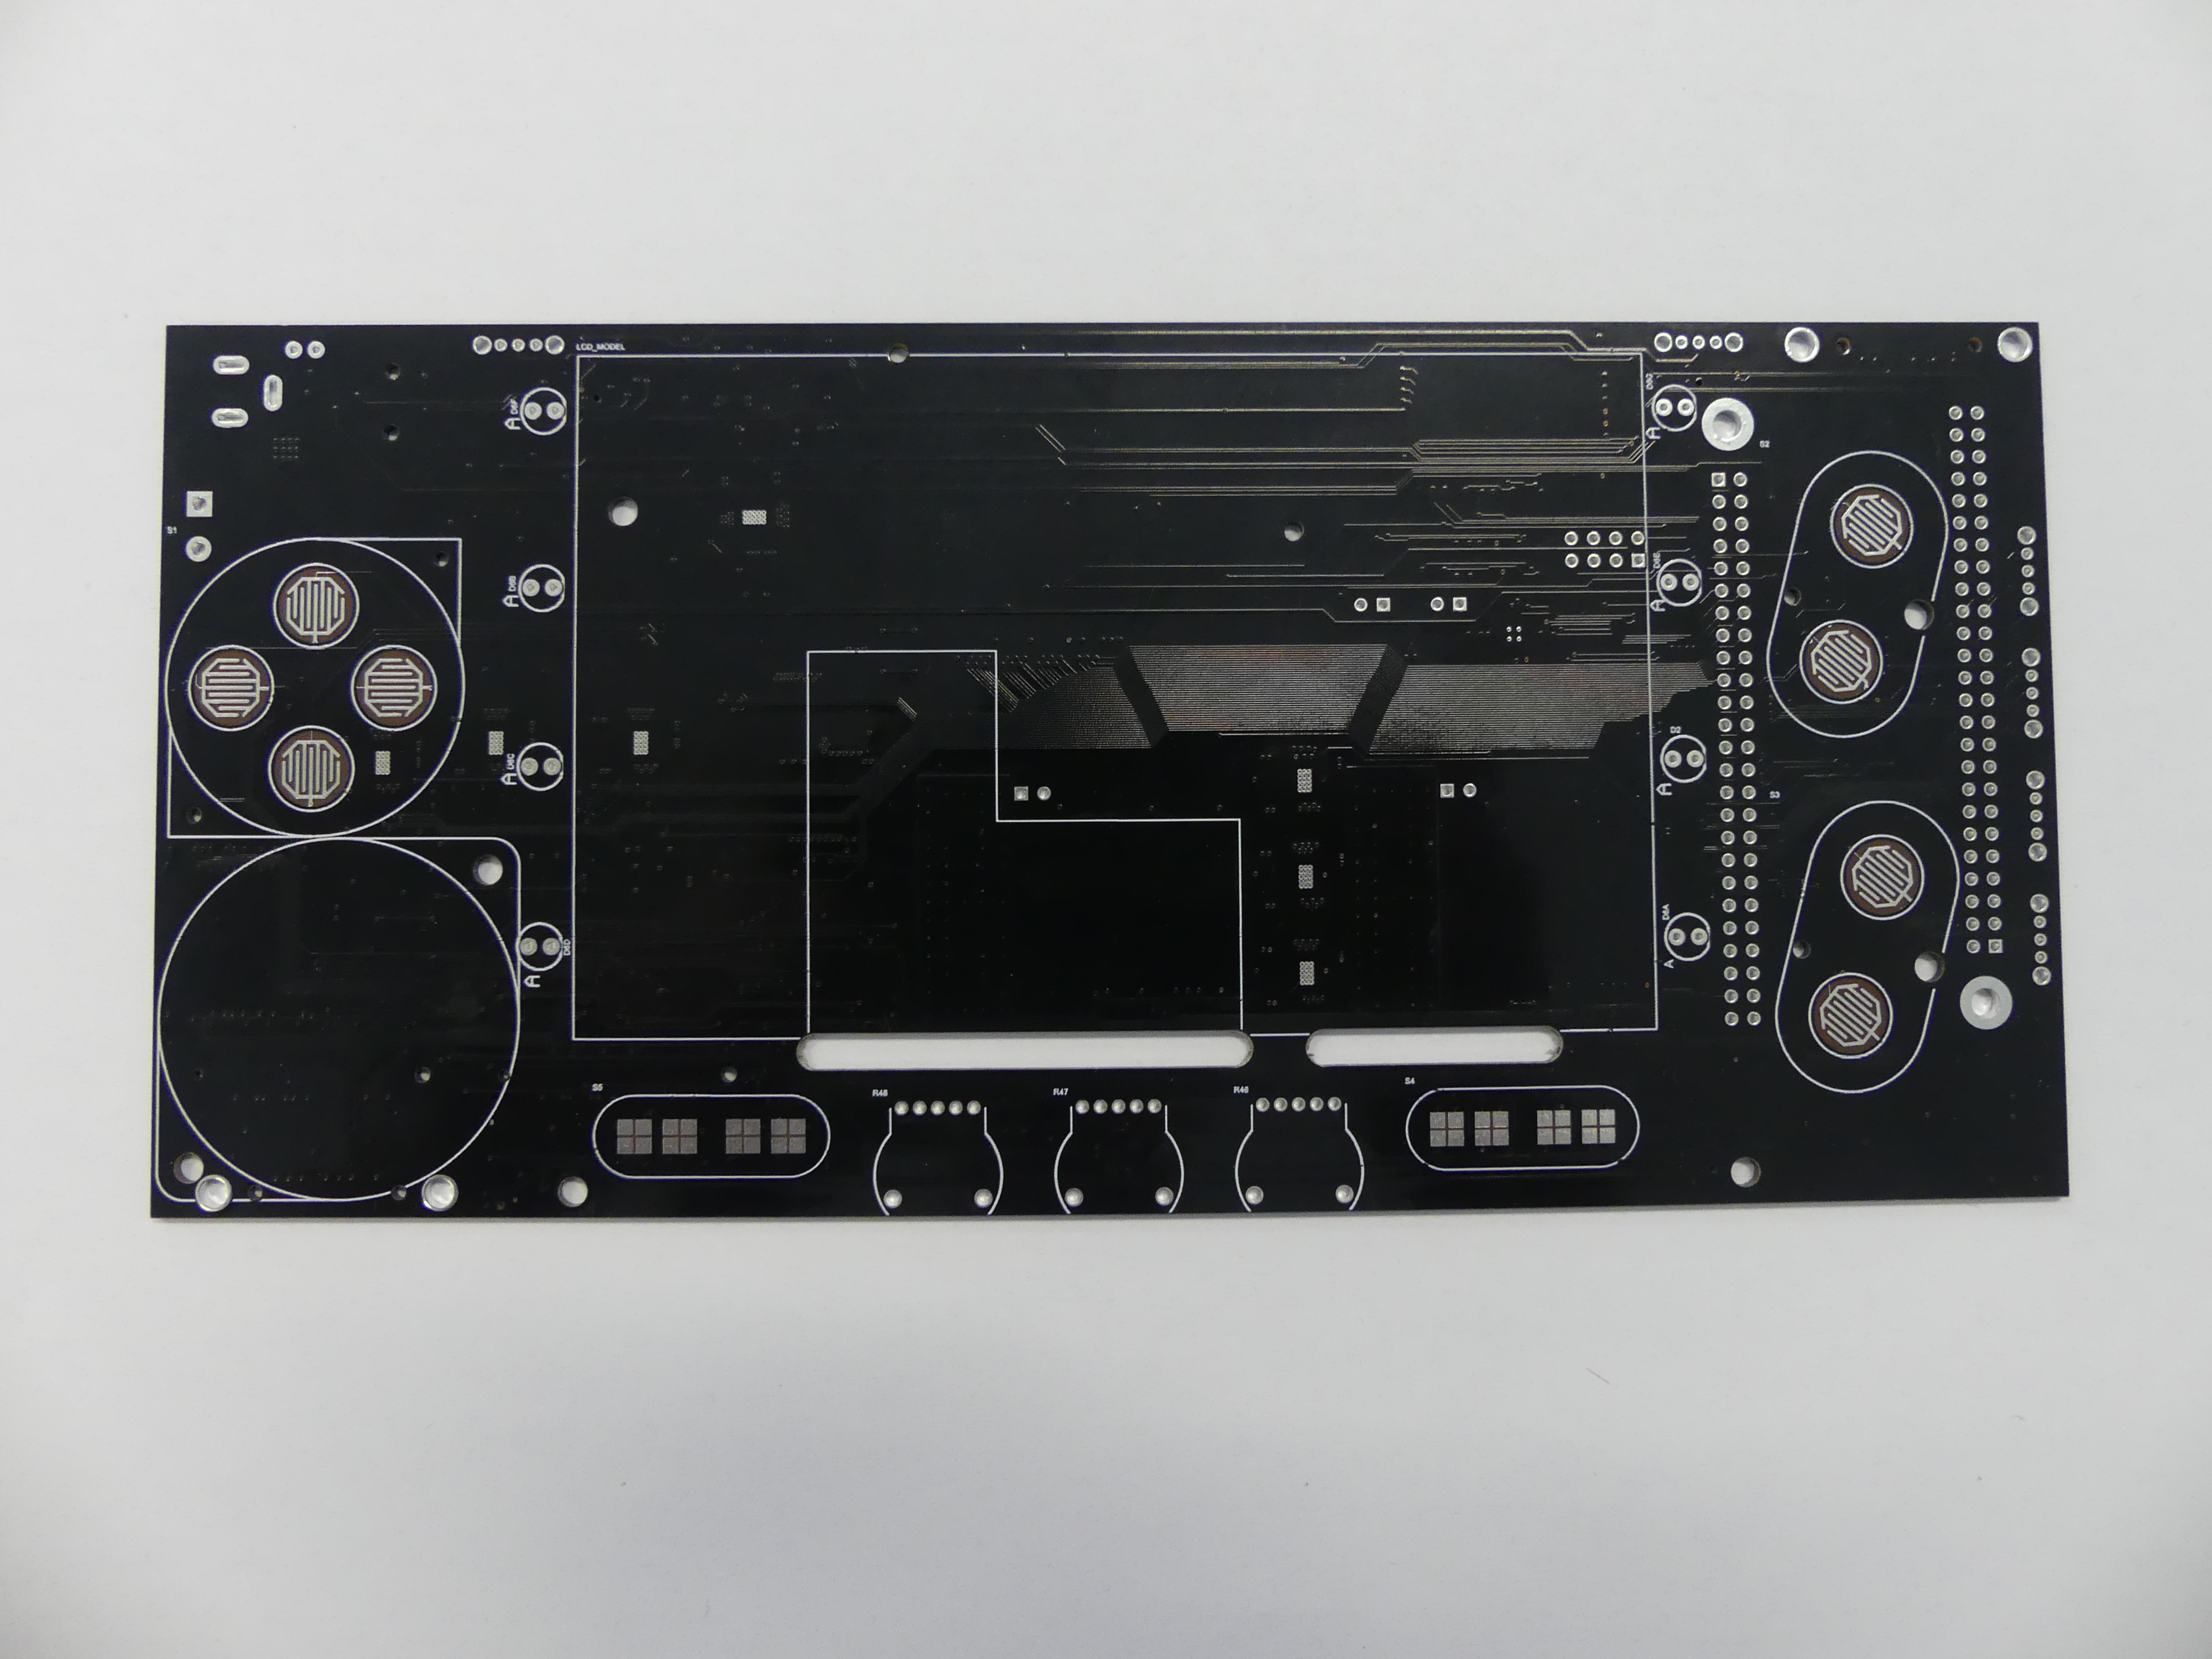
\includegraphics[width=.3\linewidth]{pics/MEGAphone_PCB_r1_empty_front} 
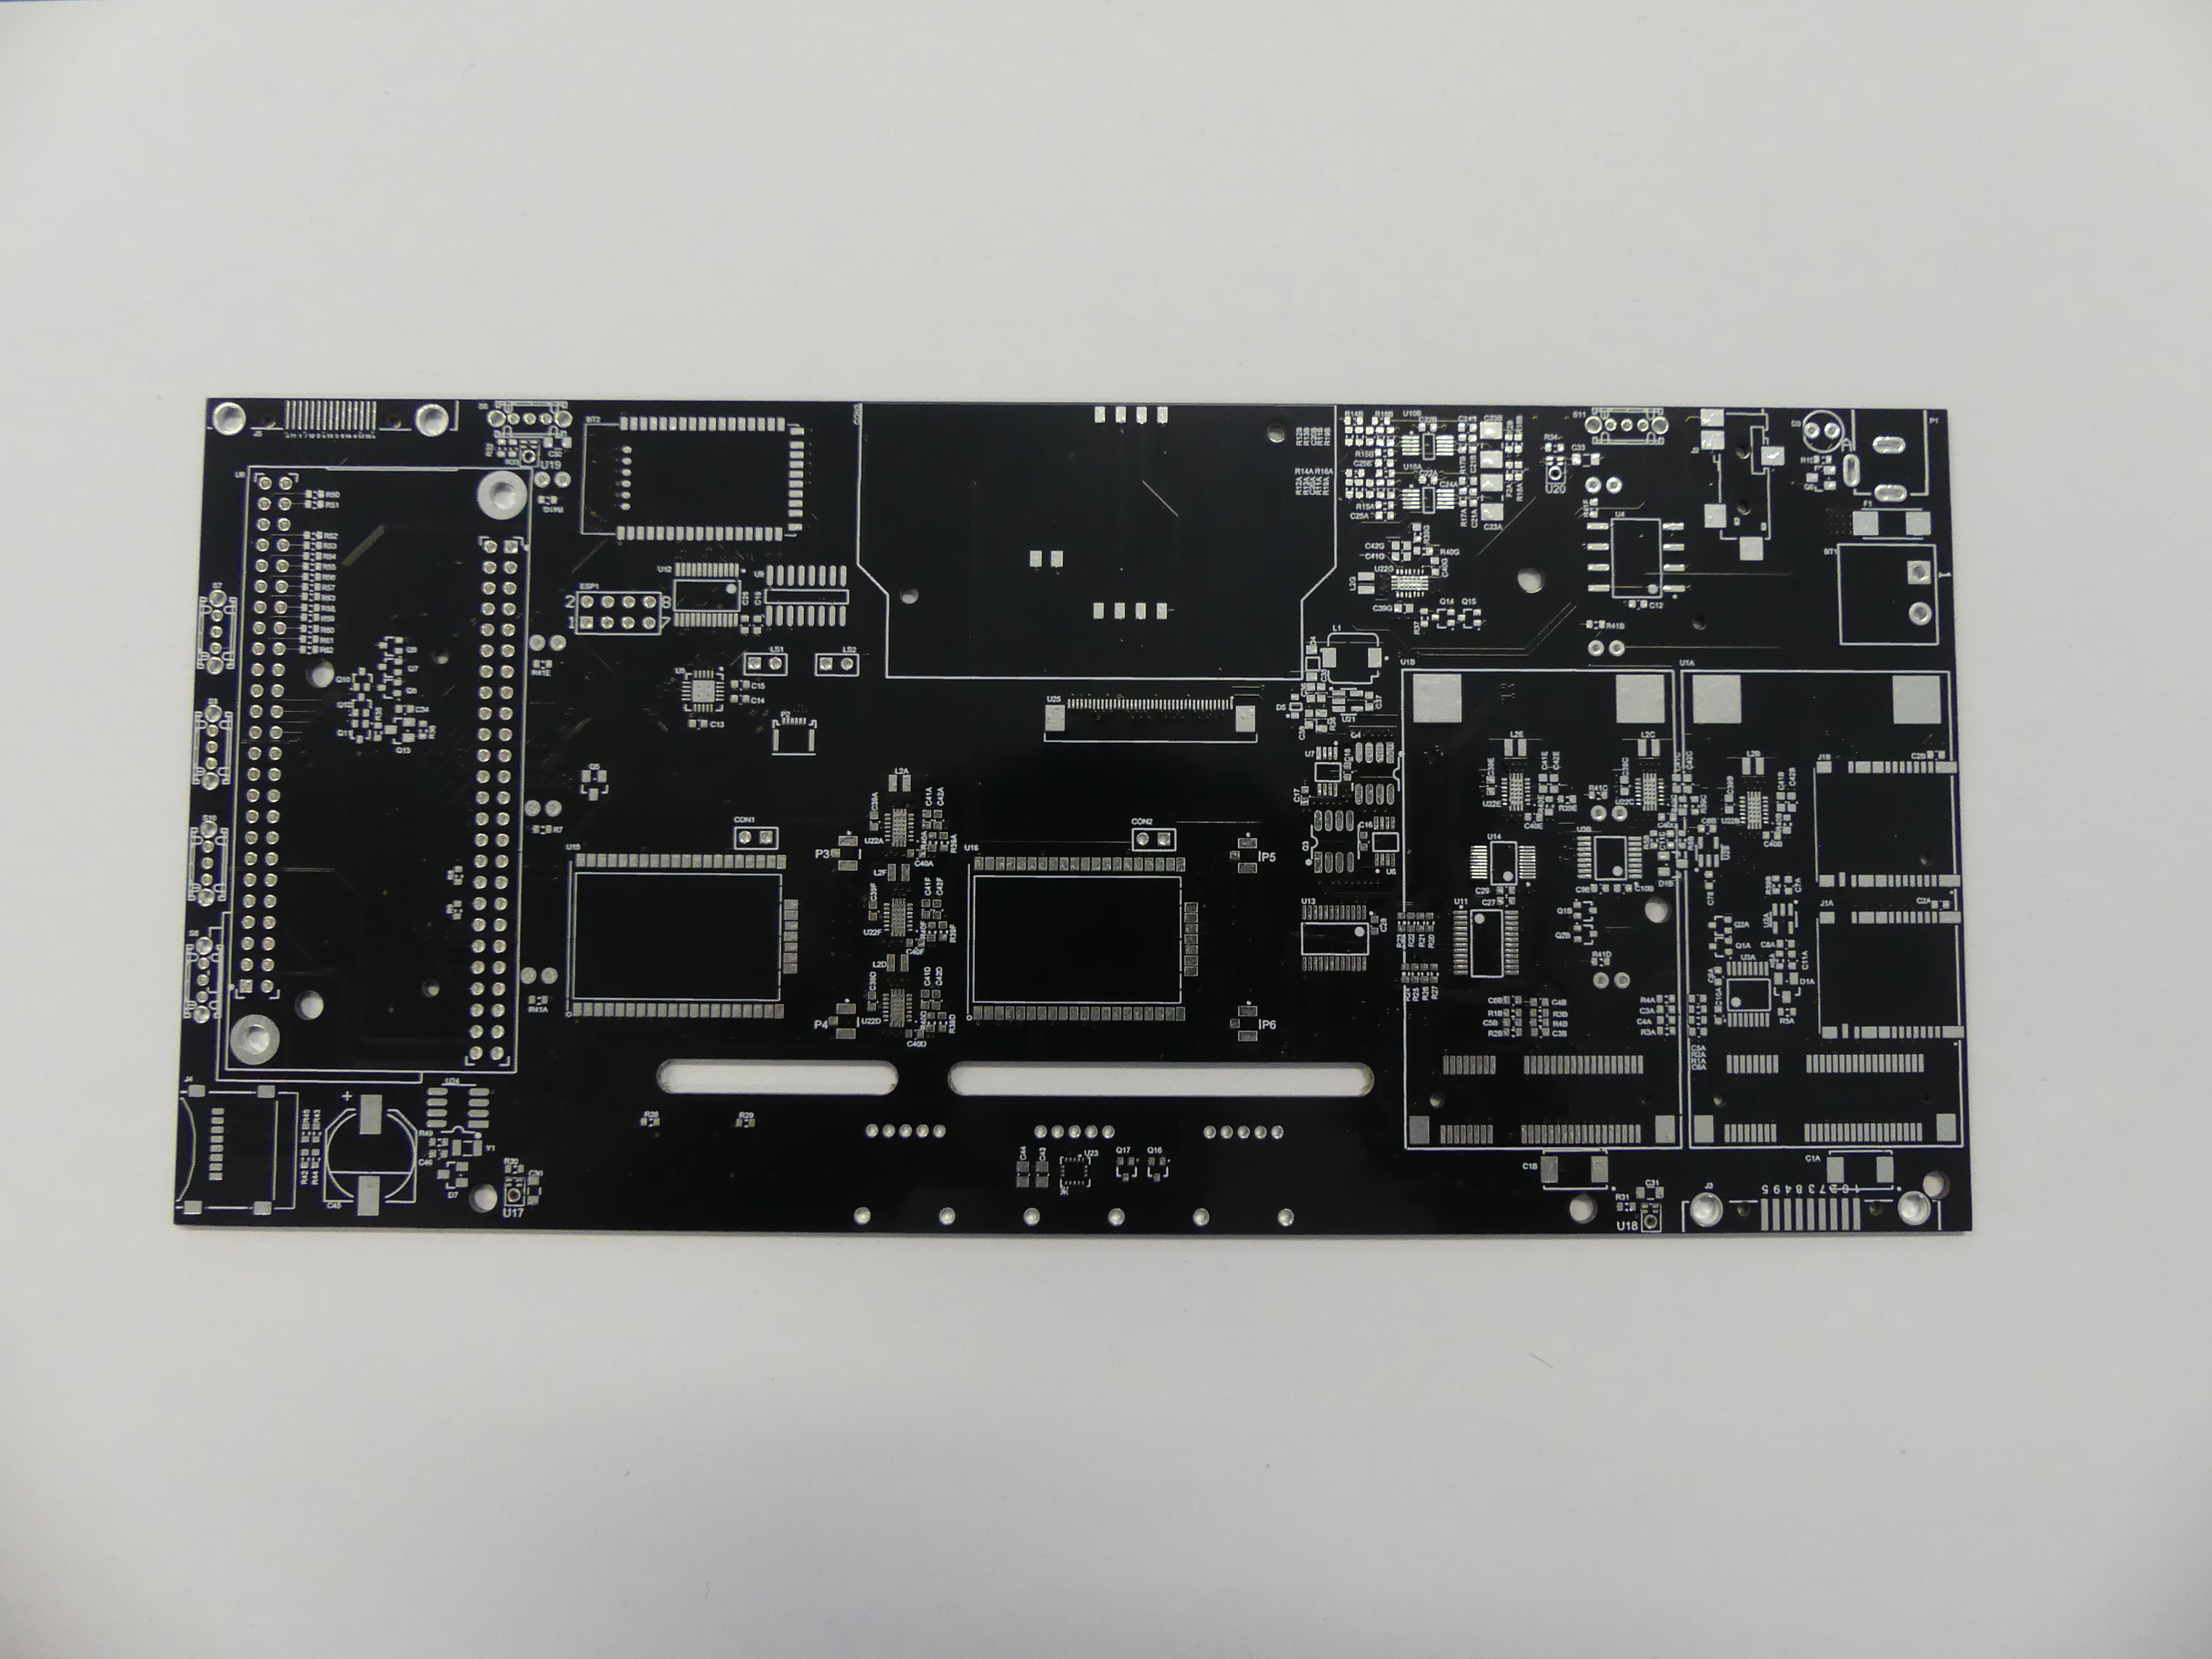
\includegraphics[width=.3\linewidth]{pics/MEGAphone_PCB_r1_empty_back} 
\end{center} 
\caption{MEGAphone PCB Revision 1 from the front and back when not populated with components. Front side is shown of the left.\\}
\label{MEGAphone_PCB_r1_empty}
\end{figure}

\begin{figure} \begin{center}
\includegraphics[width=.3\linewidth]{pics/MEGAphone_PCB_r1_populated_front} 
\includegraphics[width=.3\linewidth]{pics/MEGAphone_PCB_r1_populated_back} 
\end{center} 
\caption{MEGAphone PCB Revision 1 from the front and back populated with components. Front side is shown of the left.\\}
\label{MEGAphone_PCB_r1_populated}
\end{figure}


\textbf{Faults in Hardware}
\begin{enumerate}
\item The joystick connector, J3, is the wrong gender, currently it is female where as it should be male, figure \ref{MEGAphone_PCB_r1_J3}.
\item U1A and U1B, the footprint of the latch that holds the cellular modem is in the wrong position, figure \ref{MEGAphone_PCB_r1_U1A}.
\item U14 is not populated, this is the external joystick controller, figure \ref{MEGAphone_PCB_r1_U14}. 
\item U4 is currently missing, this is the Analogue-to-Digital converter for the microphone, figure \ref{MEGAphone_PCB_r1_U4}.
\item U25 needs to be moved a few millimetres to the right (when looking at the PCB face the component is mounted to) and also a couple of millimetres towards the slot which the ribbon runs through. This is to allow the ribbon cable to connect easier, figure \ref{MEGAphone_PCB_r1_U25}.
\item P2 need to be re-positioned a couple of millimetres towards the ribbon cable slot to allow the ribbon to connect easier \ref{MEGAphone_PCB_r1_P2}.
\item U15 may need to be moved a few millimetres to the left (when looking at the component) to allow for the ribbon cable to reach P2 without rubbing on U15 figure \ref{MEGAphone_PCB_r1_P2}.
\item LED power indicator are slightly too close together to allow the screen cover to fit between them \ref{MEGAphone_PCB_r1_LED}.
\item U9 which is the SPI flash chip, the footprint is wrong i.e. doesn't match the part, figure \ref{MEGAphone_PCB_r1_U9}.
\item R46, R47 and R48, the thumb wheels for volume control, are missing and currently on back order, figure \ref{MEGAphone_PCB_r1_R49_R48_R47}.
\item Found the PCB is outputting over 6.45 Volts where it should be outputting 3.3V. (Found to be a loose hand-soldered resistor \cite{RN162}) \\
\end{enumerate}

\begin{figure} \begin{center}
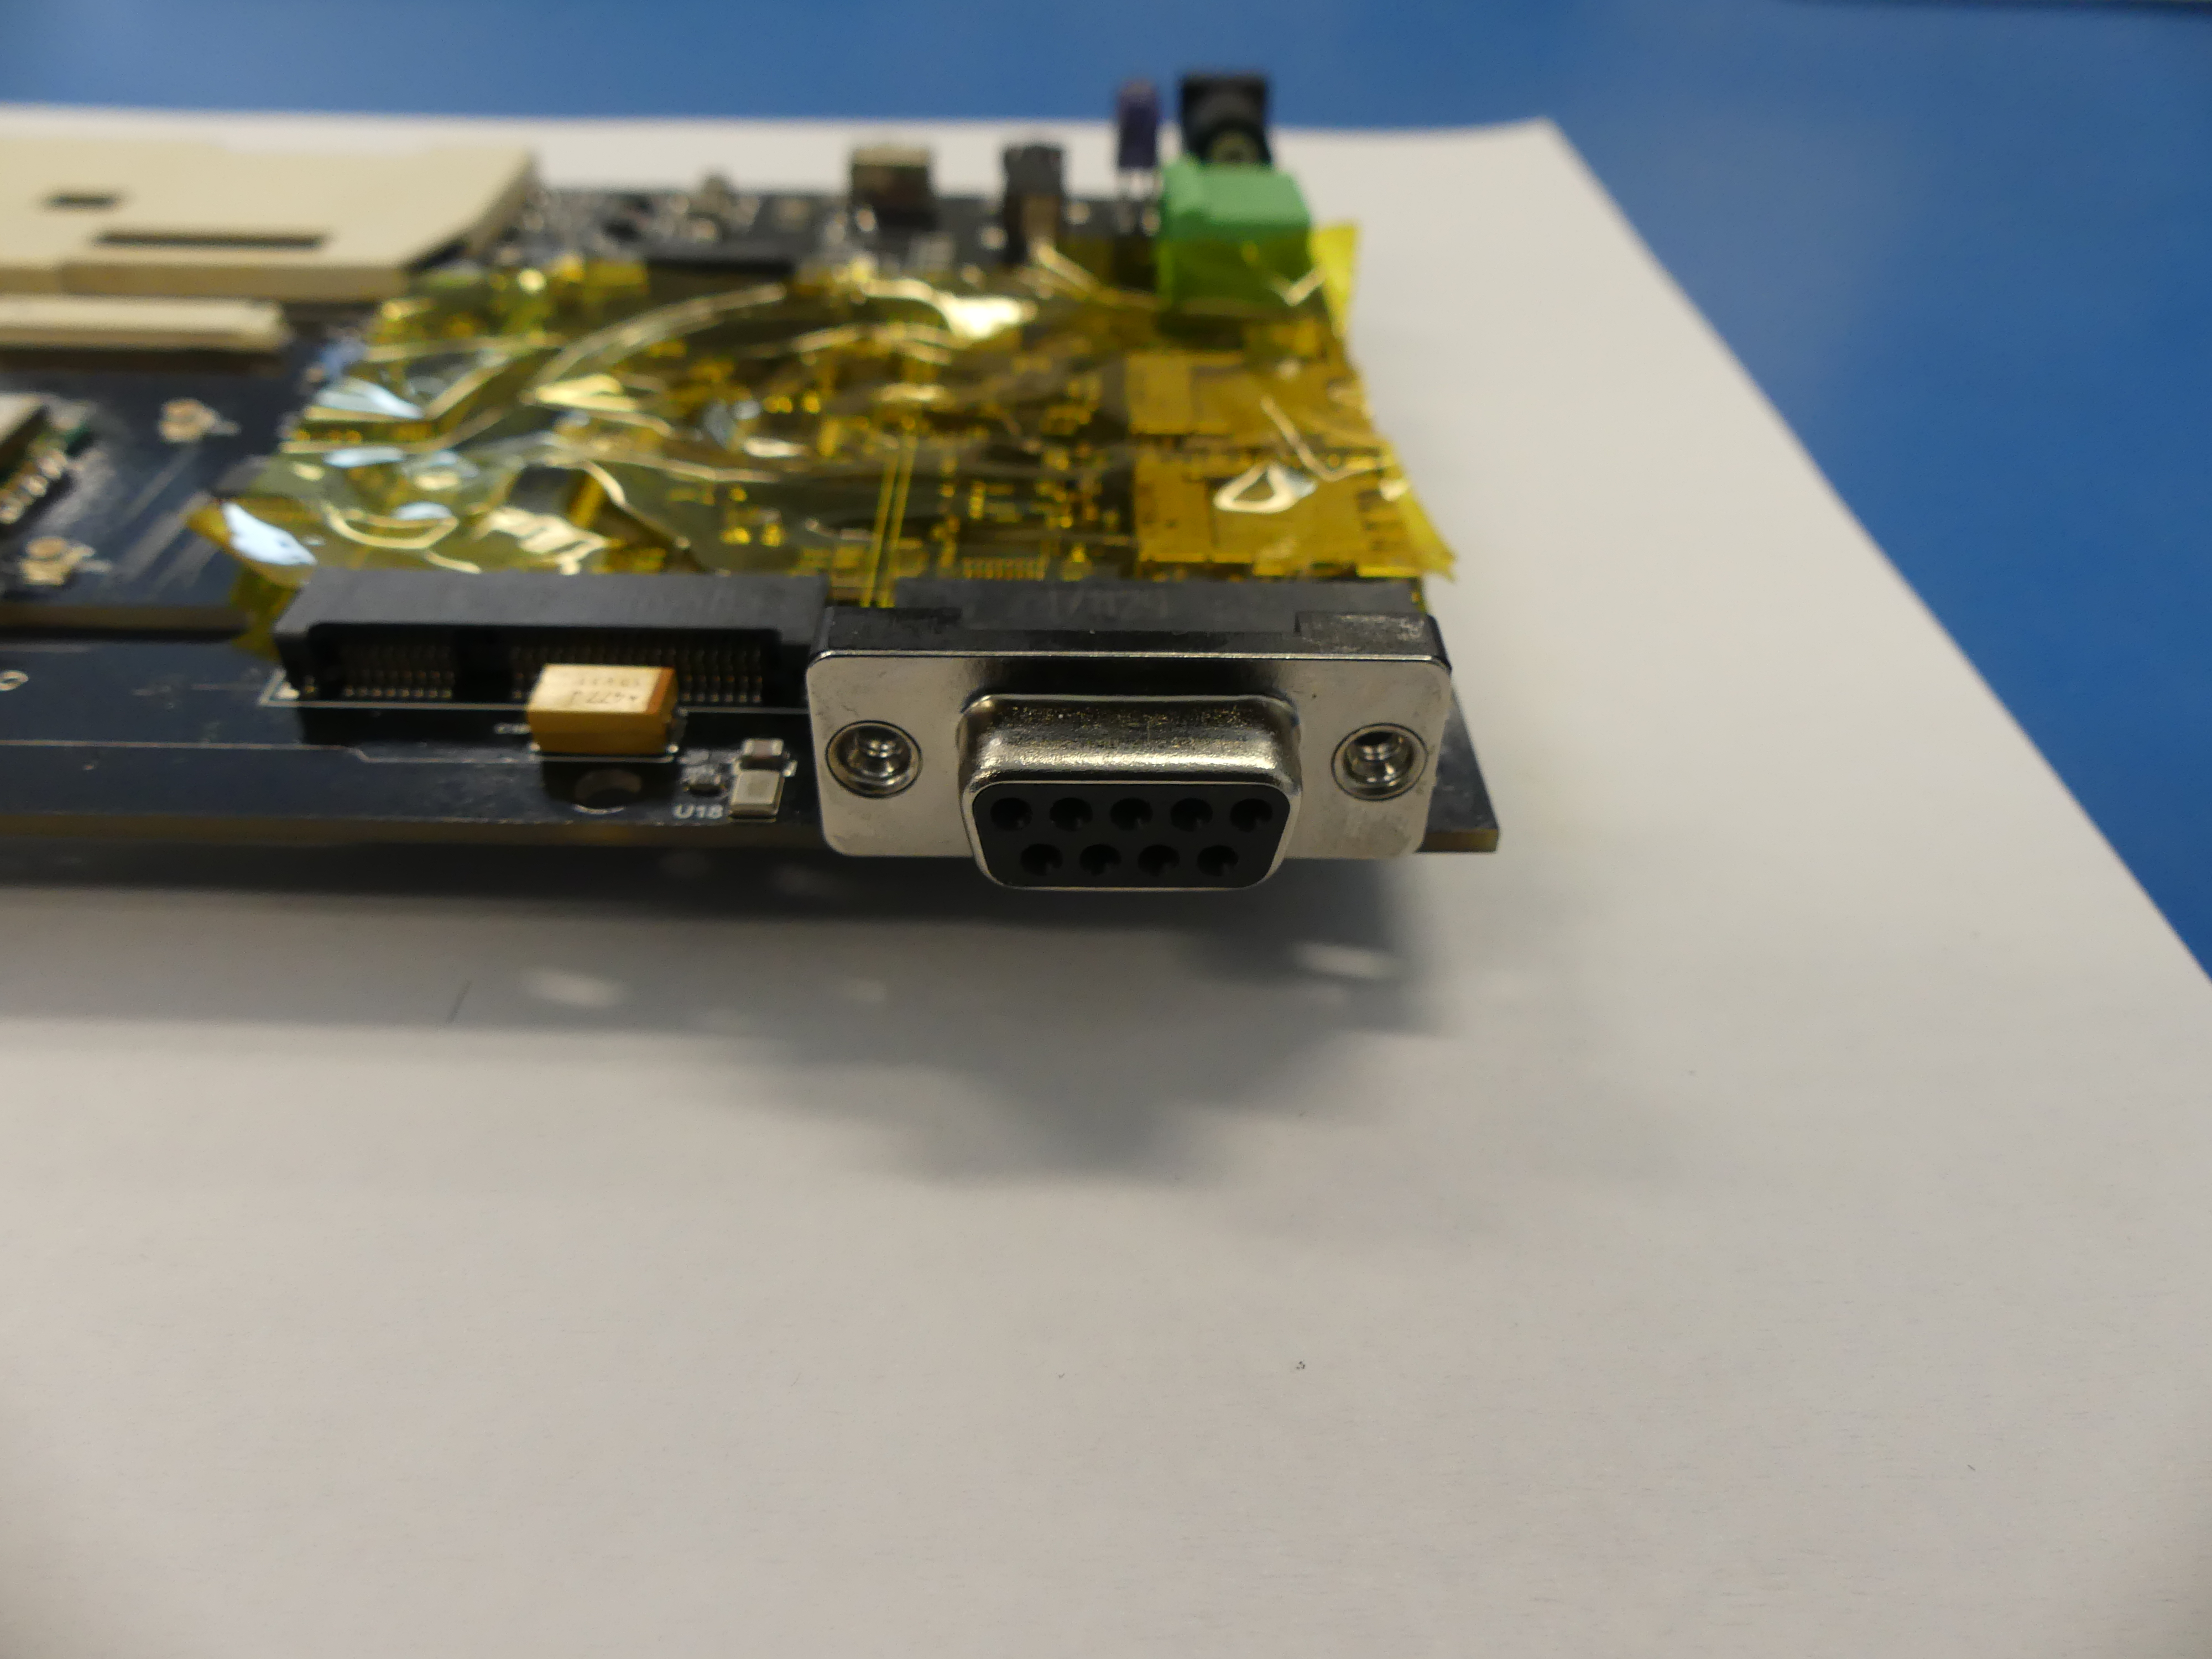
\includegraphics[width=.3\linewidth]{pics/MEGAphone_PCB_r1_J3} 
\end{center} 
\caption{Close up of Joystick connector J3, which should be a male connector.\\}
\label{MEGAphone_PCB_r1_J3}
\end{figure}

\begin{figure} \begin{center}
\includegraphics[width=.3\linewidth]{pics/MEGAphone_PCB_r1_U1A} 
\end{center} 
\caption{Close up showing the latch installed in U1B but not U1A.\\}
\label{MEGAphone_PCB_r1_U1A}
\end{figure}

\begin{figure} \begin{center}
\includegraphics[width=.3\linewidth]{pics/MEGAphone_PCB_r1_U14} 
\end{center} 
\caption{Close up showing unpopulated component U14.\\}
\label{MEGAphone_PCB_r1_U14}
\end{figure}

\begin{figure} \begin{center}
\includegraphics[width=.3\linewidth]{pics/MEGAphone_PCB_r1_U4} 
\end{center} 
\caption{Close up showing unpopulated component U4.\\}
\label{MEGAphone_PCB_r1_U4}
\end{figure}

\begin{figure} \begin{center}
\includegraphics[width=.3\linewidth]{pics/MEGAphone_PCB_r1_U25}
\includegraphics[width=.3\linewidth]{pics/MEGAphone_PCB_r1_U25_P2_ribbon}
\end{center} 
\caption{Close up showing component U25 as well with as the ribbon connector for the screen. U25 needs to be re-positioned.\\}
\label{MEGAphone_PCB_r1_U25}
\end{figure}

\begin{figure} \begin{center}
\includegraphics[width=.3\linewidth]{pics/MEGAphone_PCB_r1_P2}
\includegraphics[width=.3\linewidth]{pics/MEGAphone_PCB_r1_U25_P2_ribbon}
\end{center} 
\caption{Close up showing component P2 as well with as the ribbon connector for the screen. P2 needs to be re-positioned. \\}
\label{MEGAphone_PCB_r1_P2}
\end{figure}

\begin{figure} \begin{center}
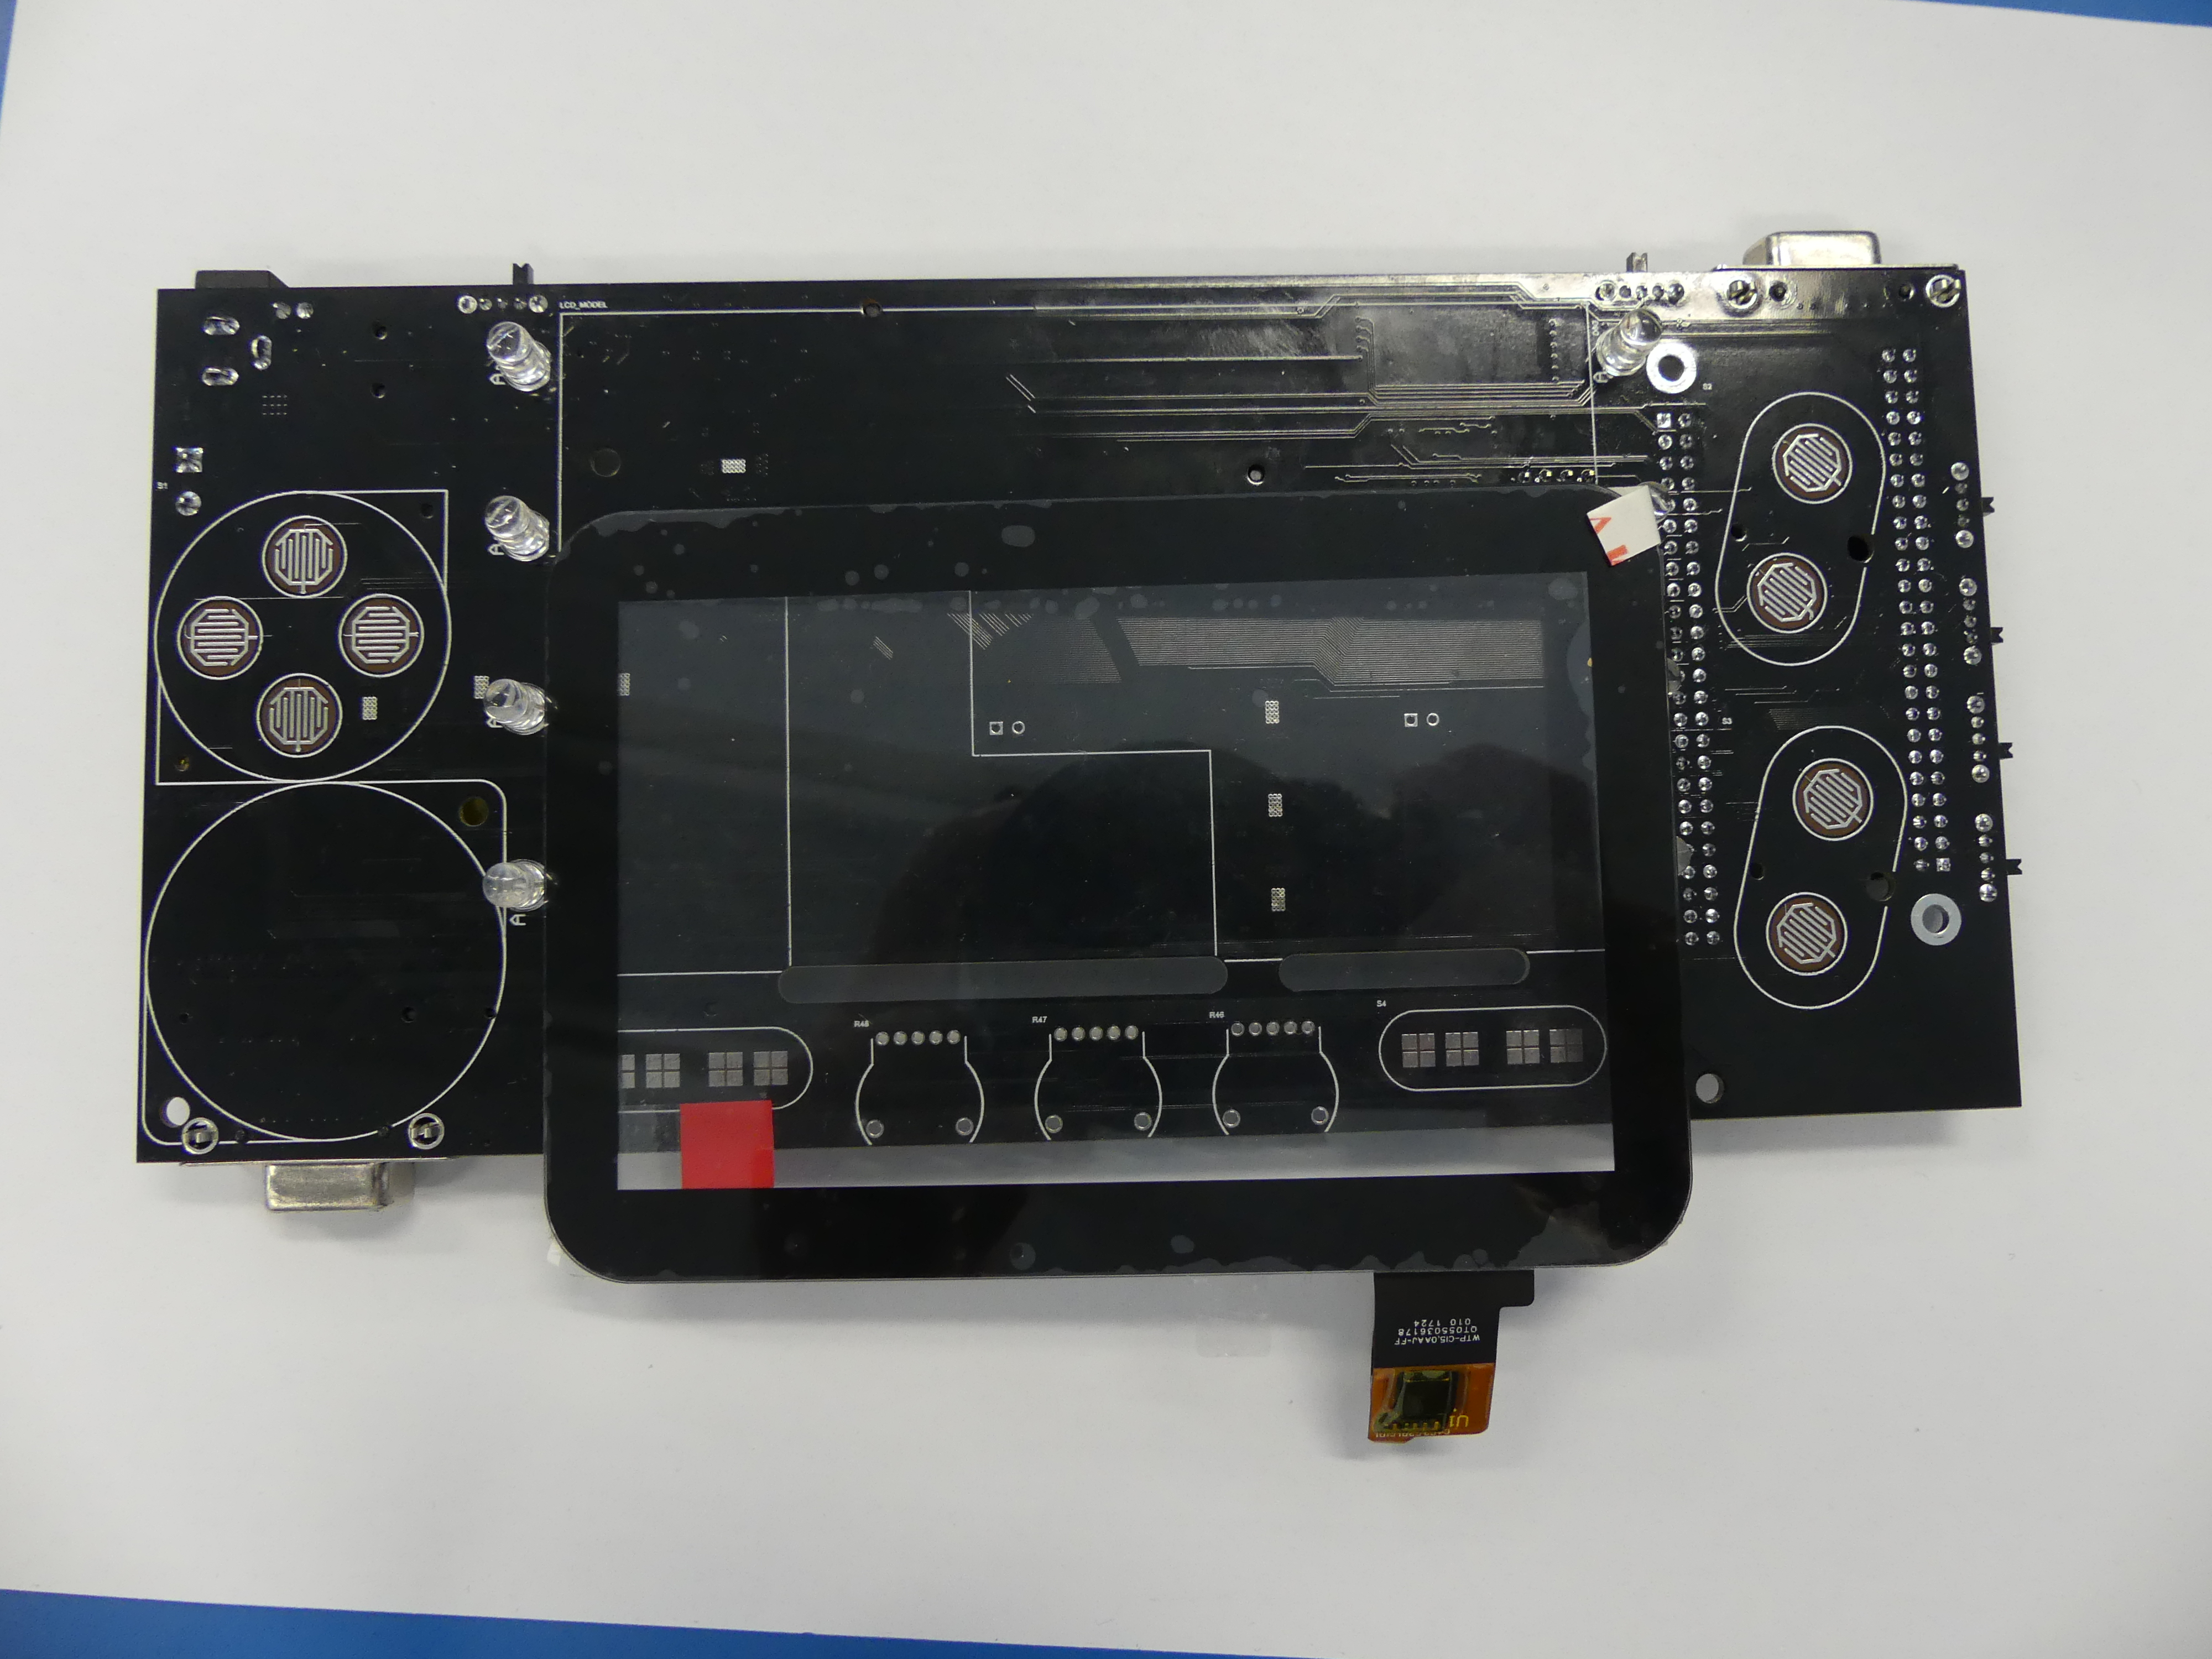
\includegraphics[width=.3\linewidth]{pics/MEGAphone_PCB_r1_LED1}
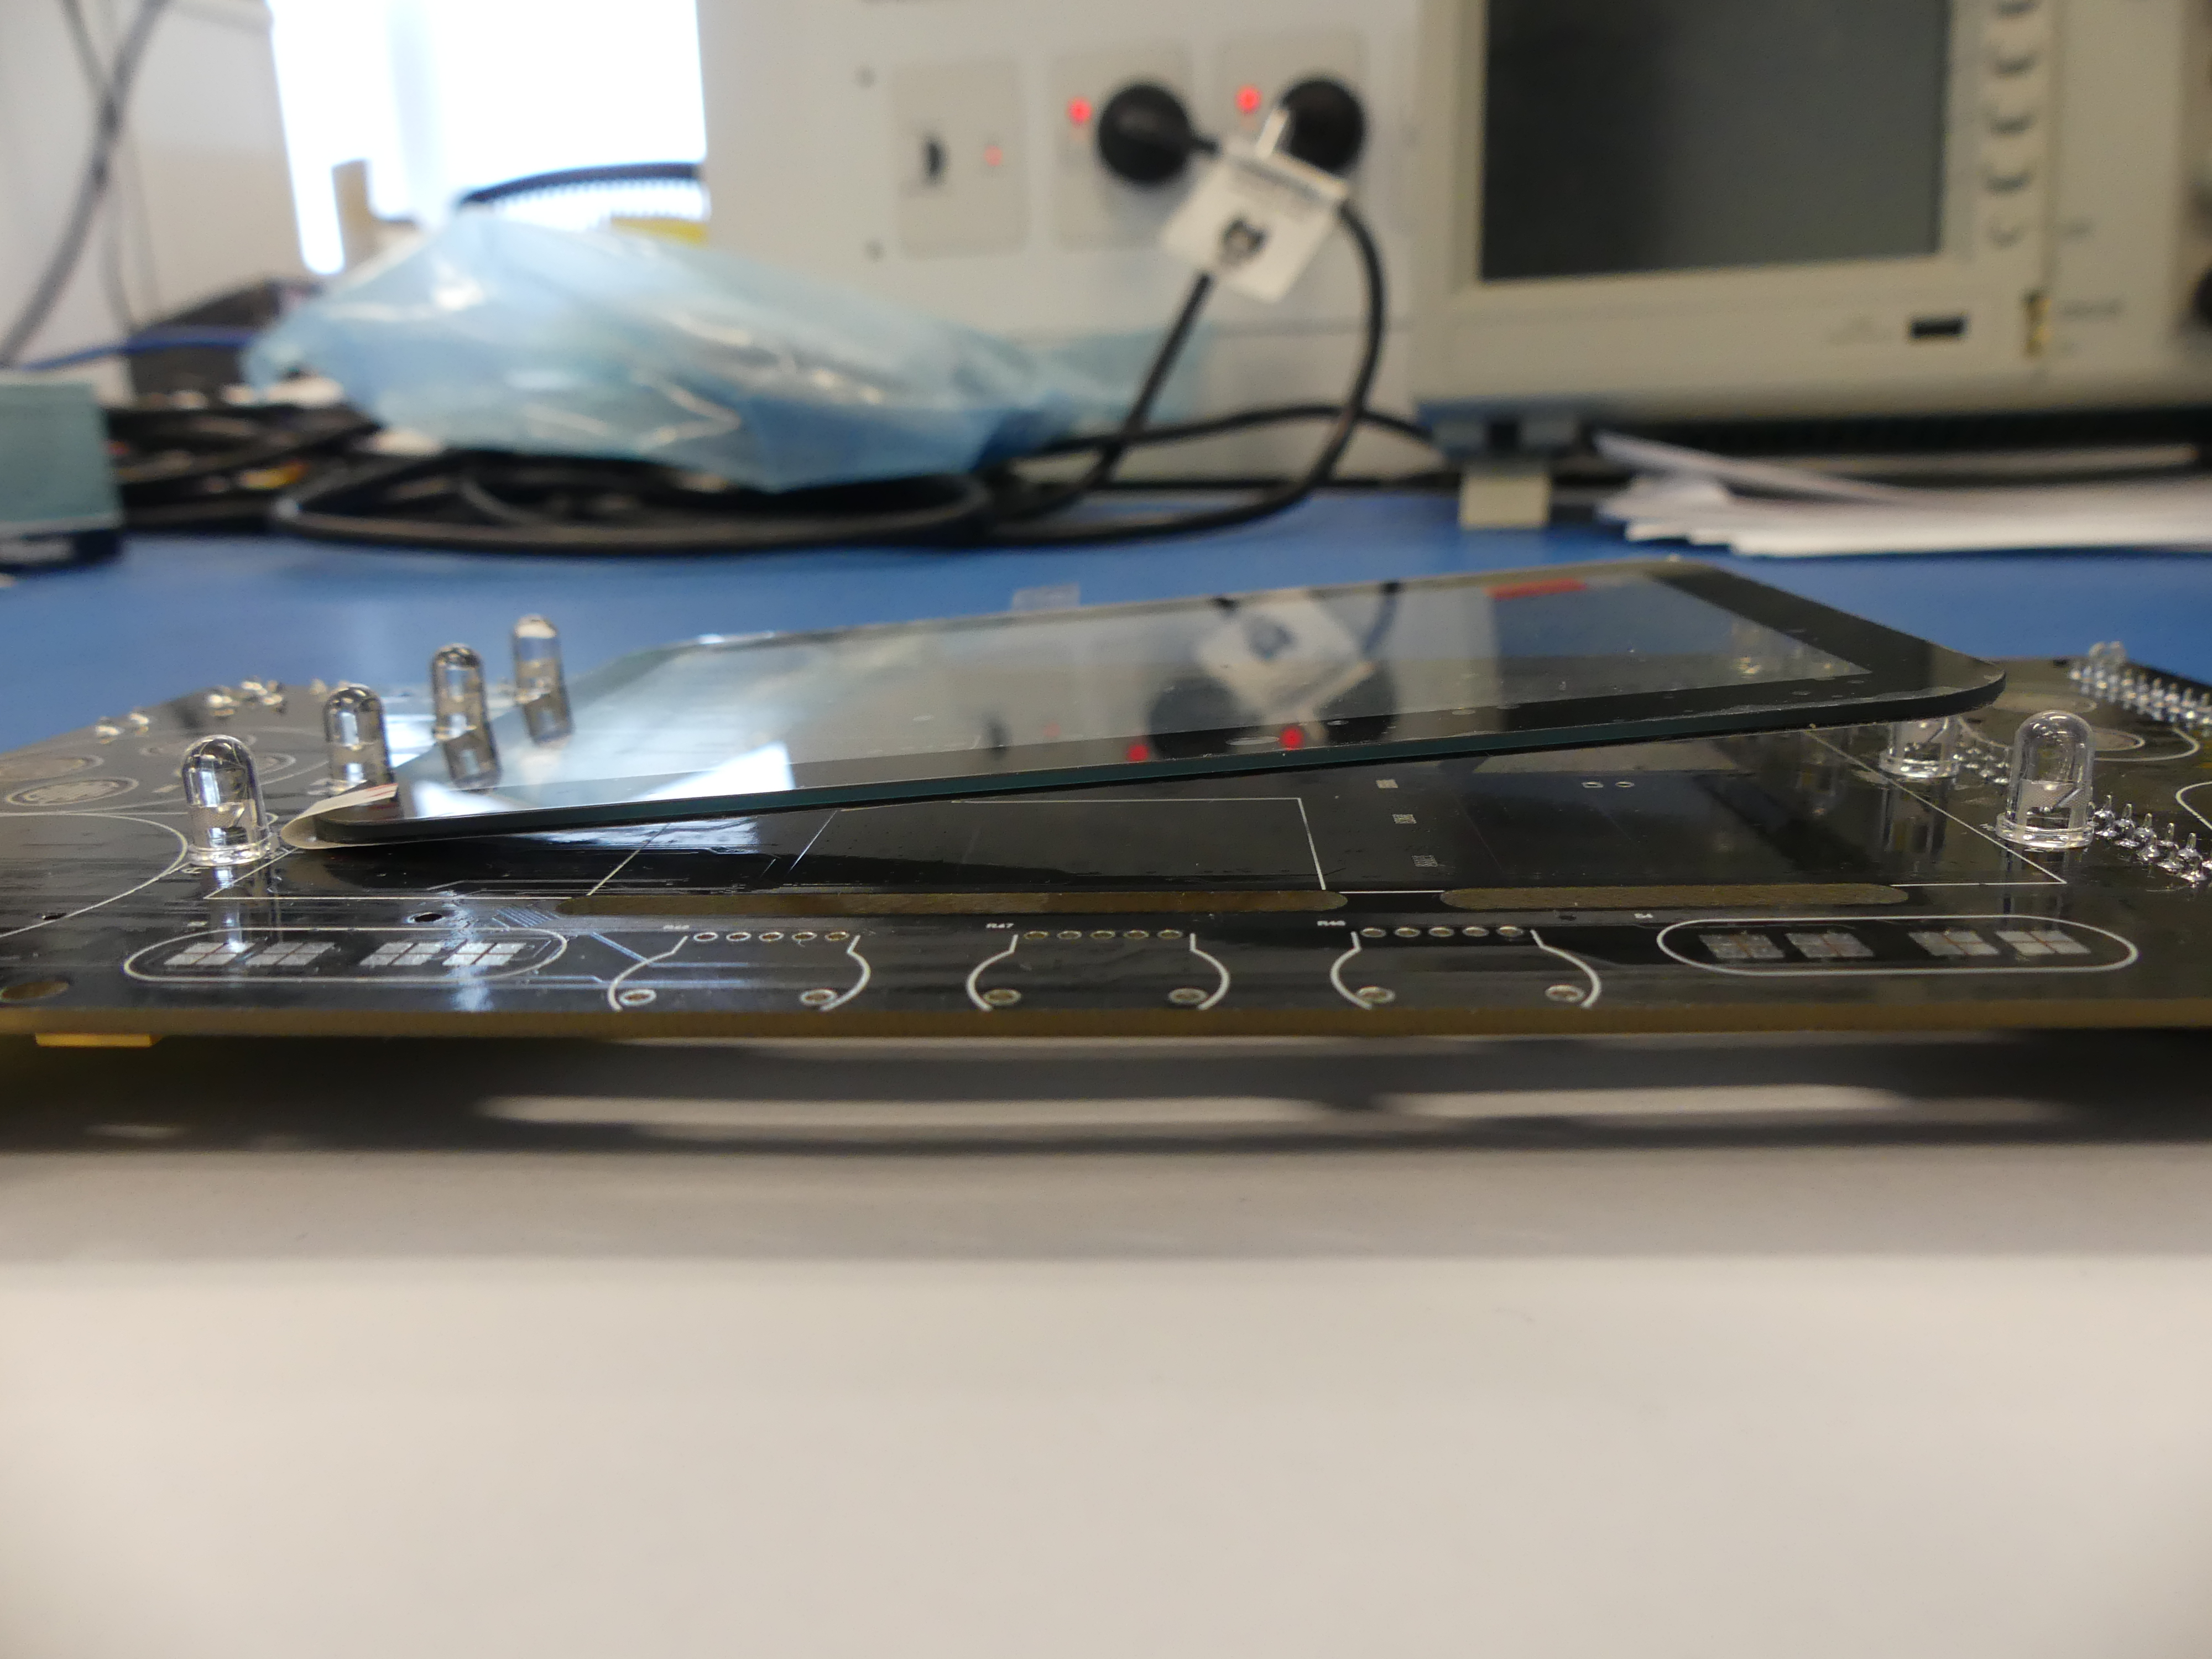
\includegraphics[width=.3\linewidth]{pics/MEGAphone_PCB_r1_LED2}
\includegraphics[width=.3\linewidth]{pics/MEGAphone_PCB_r1_LED3}
\end{center} 
\caption{Close up showing position of LED on front face of PCB. Screen cannot fit between them. \\}
\label{MEGAphone_PCB_r1_LED}
\end{figure}

\begin{figure} \begin{center}
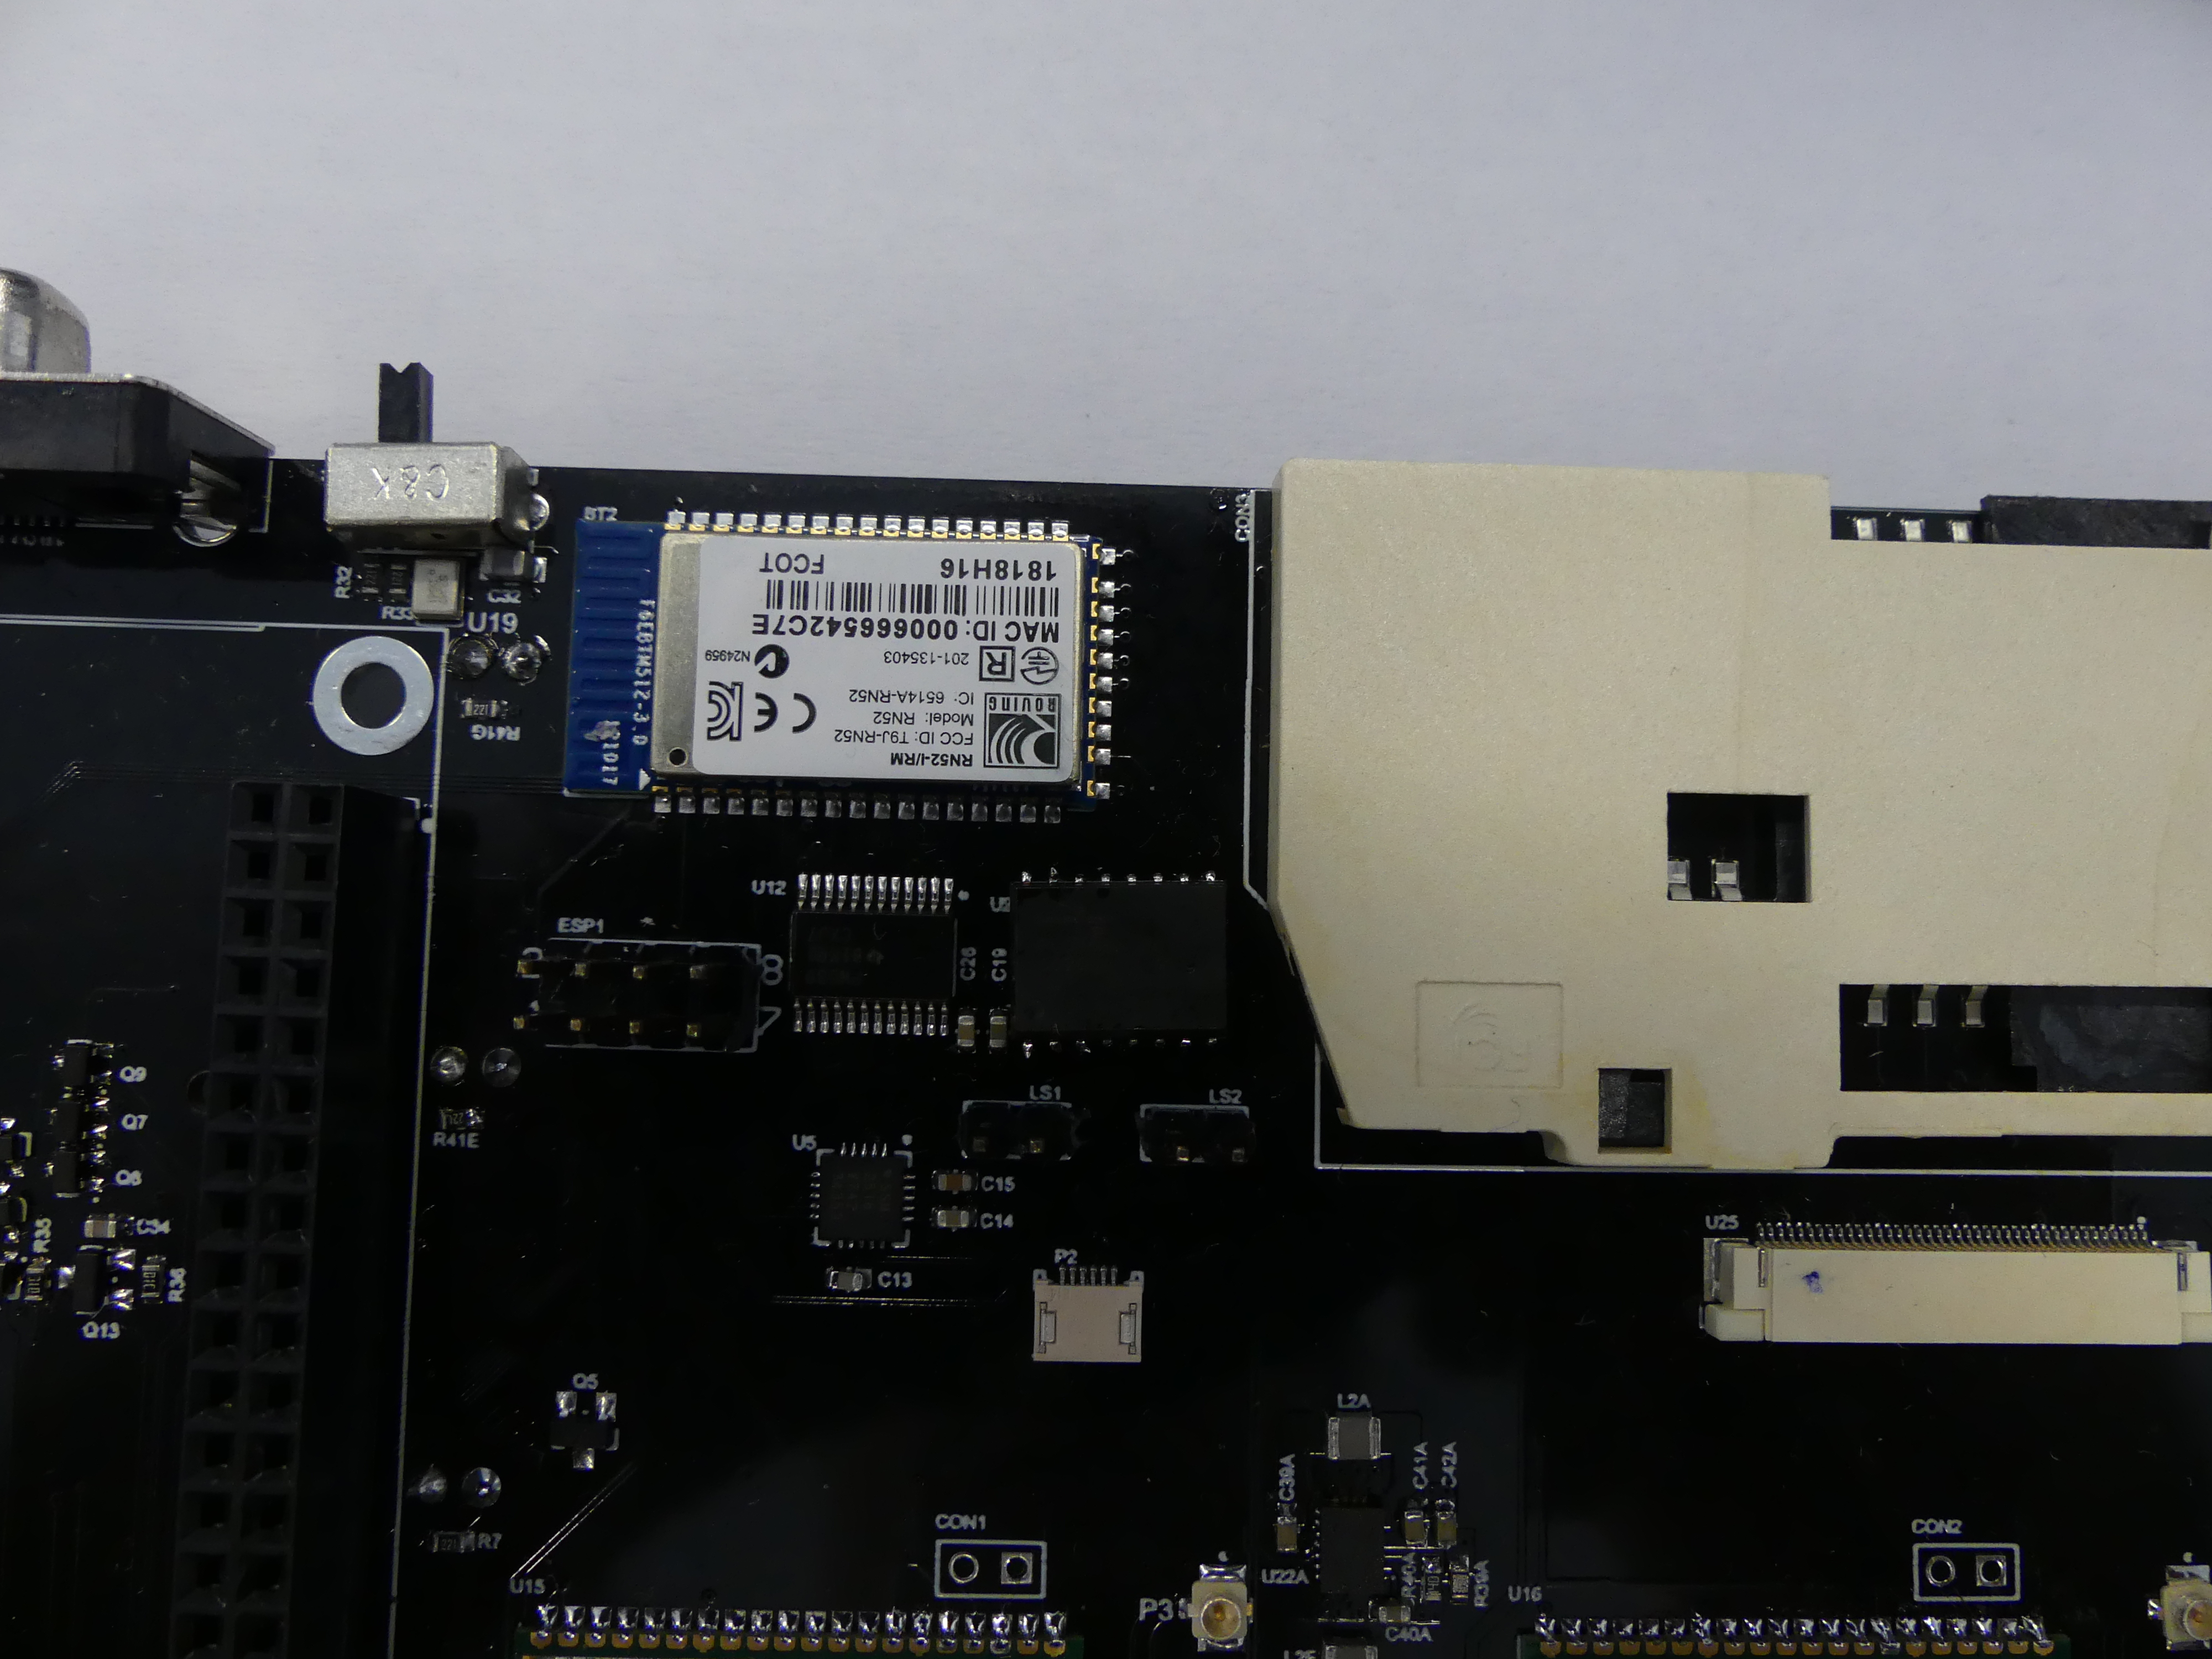
\includegraphics[width=.3\linewidth]{pics/MEGAphone_PCB_r1_U9}
\end{center} 
\caption{Close up of U9 which didn't fit its footprint and had to be modified to fit. \\}
\label{MEGAphone_PCB_r1_U9}
\end{figure}

\begin{figure} \begin{center}
\includegraphics[width=.3\linewidth]{pics/MEGAphone_PCB_r1_R48_R47_R46}
\includegraphics[width=.3\linewidth]{pics/MEGAphone_PCB_r1_populated_front}
\end{center} 
\caption{Close up of missing thumb wheels for volume control, R46, R47 and R48. \\}
\label{MEGAphone_PCB_r1_R49_R48_R47}
\end{figure}

\textbf{Things that need to be tested}
\begin{enumerate}
\item U1A and U1B, might not have enough clearance to fit the cellular modems in place due to components mounted on PCB in this area. 4G modem component to be used to test if it fits. Components within U1A and U1B footprint may need to be relocated if the 4G modem doesn't fit. In particular, the components J1A and J1B may need to be lower profile connectors such as a SIM card connector without the microSD slot above it, which it currently has on both J1A and J1B. Shown in figure \ref{MEGAphone_PCB_r1_U1A_clearance} \\
\end{enumerate}

\begin{figure} \begin{center}
\includegraphics[width=.3\linewidth]{pics/MEGAphone_PCB_r1_U1A_clearance1}
\includegraphics[width=.3\linewidth]{pics/MEGAphone_PCB_r1_U1A_clearance2}
\end{center} 
\caption{Close up of clearance above U1A and U1B footprints, a cellular modem needs to be inserted in this space. \\}
\label{MEGAphone_PCB_r1_U1A_clearance}
\end{figure}


\textbf{Components or functions which cannot be tested currently}
\begin{enumerate}
\item Microphone audio.
\item Thumb wheels for volume control, R48, R47 and R46.
\item 2nd PCIe modem slot, U1A.
\item 2nd SIM card slot, associated with the 2nd modem, U1A, mentioned above.
\item The ribbon cable connections between U25, P2 and the screen cannot be fully tested with the screen in position but a partial test with the screen offset should be possible.
\item Speaker currently not installed but parts and component are present in lab. \\
\end{enumerate}

\textbf{Noteworthy feature}
\begin{enumerate}
\item Installation of insulating tape covering components within the U1A and U1B footprints. This is to provide insulation between conductive part of components and the modem which will be inserted above them, seen in figure \ref{MEGAphone_PCB_r1_U1A_clearance} and \ref{MEGAphone_PCB_r1_U14}. \\
\end{enumerate}

LED 5mm high. screen 3mm high. lead sitcking up are 1mm high.

2 x 1 mm layers of spacers - 1 with holes for leads one without

\subsection{Other Components}


%----------------------------------------------------------------------------------------
%----------------------------------------------------------------------------------------
\section{MEGA65 Desktop Computer Form Factor}
This section looks at the current state of the MEGA65 Desktop form-factor. The Desktop form-factor's physical development is being overseen by M.E.G.A. in Germany. The physical development refers to the electronics hardware, case and keyboard. It still uses the same FPGA-based core, developed by Dr Gardner-Stephens, as the MEGAphone. Following a discussion the Detlef in Germany, who is overseeing the development of the MEGA65 Desktop, the following state of the MEGA65 Desktop hardware was elicited. 

The MEGA65 Desktop is currently in a "pre-series" stage, the machines are roughly 95\% complete and have been created in their current state so they can be tested in a real-life environment. 

\subsection{Case}
The current case has had a few modifications from the original design, which was based on the Commodore 65 case. It has a new appearance with a original case design which has been described as "cleaner". The new case also has some major changes around the port at the back of the computer and some minor changes to the trapdoor on the bottom as well as some additions for ventilation. These design changes to the new case where carried out by Hintsteiner in Austria.

The MEGA65 Desktop is planned for a pre-production run of 20 machines using the new case design. This run will use vacuum moulds for the cases to reduce costs but the vacuum mould process has some drawbacks: 
\begin{enumerate}
\item The mould will only only be bale to create 20 cases before it has to be replaced.
\item The colour of the plastic forming the case slightly changes between cases.
\item Some parts of the case need to be manually fixed after the vacuum mould adding costs and the need to paint sections of the case.
\end{enumerate}

*PIC OF NEW CASE TO COME FROM DETLEF*

\subsection{Keyboard}
The keyboard for the MEGA65 Desktop is being produced by GMK, a German company. It features Cherry MX mechanical switches and 2 embedded metal plates, intended to provide very high stability. There are 2 LEDs for the lock keys, capslock and numlock and 4 RGB LEDs for power and floppy activity indicators, these are all powered by a custom-made communication bus. The keyboard also has a CPLD-based controller in place of the more widely used ARM7 microcontroller, this was done intentional to avoid "having more intelligence inside the keyboard than inside the computer".

Detlef has ordered 25 keyboards for the pre-production run, this was intentionally more than the 20 cases being produced, as mentioned above. It will provide for 5 case-less machines to use as spare-parts. It is expected that the keyboards will be in a finished state and require no more design work 

\subsection{PCB}
The PCB provides the interface between the FPGA architecture and the physical circuitry required for such features as the LEDs, I/O ports, speakers and keyboard. The design of the PCB for the MEGA65 Desktop version is being carried out by Antii Lukats at Trenz Elektronik. Currently Lukats is working on the 'r2' version of the PCB and it should be finished in early April, 2019. From there a pre-production run of 25 will be manufactured and then populated with components, before being send to Detlef. 

During the design of the PCB, a challenge arose from the need to combine modern components with much older components such as the floppy disk connector and the 9-pin joystick port. This required a larger number of different voltage levels to power the components than a purely modern component machine. 

\subsection{Other Components}
To make a finished product the MEGA65 will need more than the computer its self, there also needs to be considerations and preparations made for such things as the box, manual, silica gel for packing, warning and warranty paperwork and CE certification paperwork. To complete the computer itself also requires some extra items such as serial number stickers, warranty seals/stickers, type signs, power supply units, screws, SD card, floppy drives and cables.